\title{Mapeamento do Solo}
\subtitle{É Possível Mapear \textit{Abstrações}?}
\author{por Alessandro Samuel-Rosa}
\maketitle




\begin{wrapfigure}{l}{0.15\textwidth}
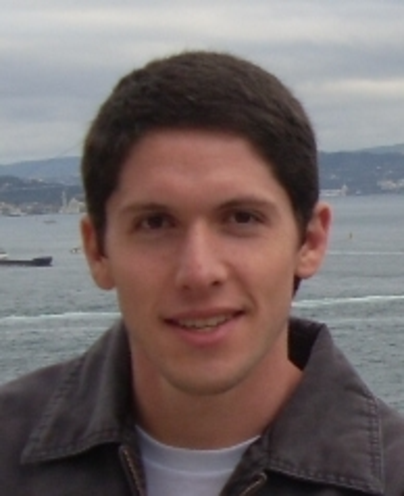
\includegraphics[width=0.15\textwidth]{figuras/alessandro}
\end{wrapfigure}




O que mapeamos quando fazemos um levantamento de solos? Essa pergunta parece ser de fácil resposta. Entretanto, se pararmos para pensar um pouco veremos que a resposta não é assim tão fácil de ser elaborada. Isso porque não há - e nunca haverá - consenso sobre o conceito de solo. Segundo David Rossiter, existem inúmeras respostas à pergunta acima. Quando fazemos um levantamento de solos podemos mapear as condições das terras, apenas o solo (conforme a definição de solo usada), o solo e algumas condições superficiais intimamente ligadas à ele, entre outras possibilidades \citep{Rossiter2000}.




Nos últimos anos, tem sido comum encontrar mapas de solo que apresentam a distribuição espacial de classes taxonômicas do solo de acordo com algum sistema nacional ou internacional de classificação do solo. Tais mapas são diferentes dos tradicionais mapas de solo que pautam-se pelo delineamento de unidades de mapeamento cujos limites são definidos pelas características das terras sendo mapeadas (isso inclui o relevo, a vegetação, a geologia, e o solo, é claro, entre outros aspectos). O exemplo mais recente de mapa de classes taxonômicas, neste caso das classes taxonômicas do WRB - World Reference Base for Soil Resources \citep{fao2007}, é o mapa publicado em meio digital no último mês de dezembro como fruto do projeto Global Soil Information Facilities, do ISRIC - World Soil Information, em parceria com a FAO e a Aliança Global pelo Solo (Figura \ref{fig:worldgrids}).




\begin{figure*}[tb!]
\begin{minipage}[t]{1\linewidth}
\begin{center}
 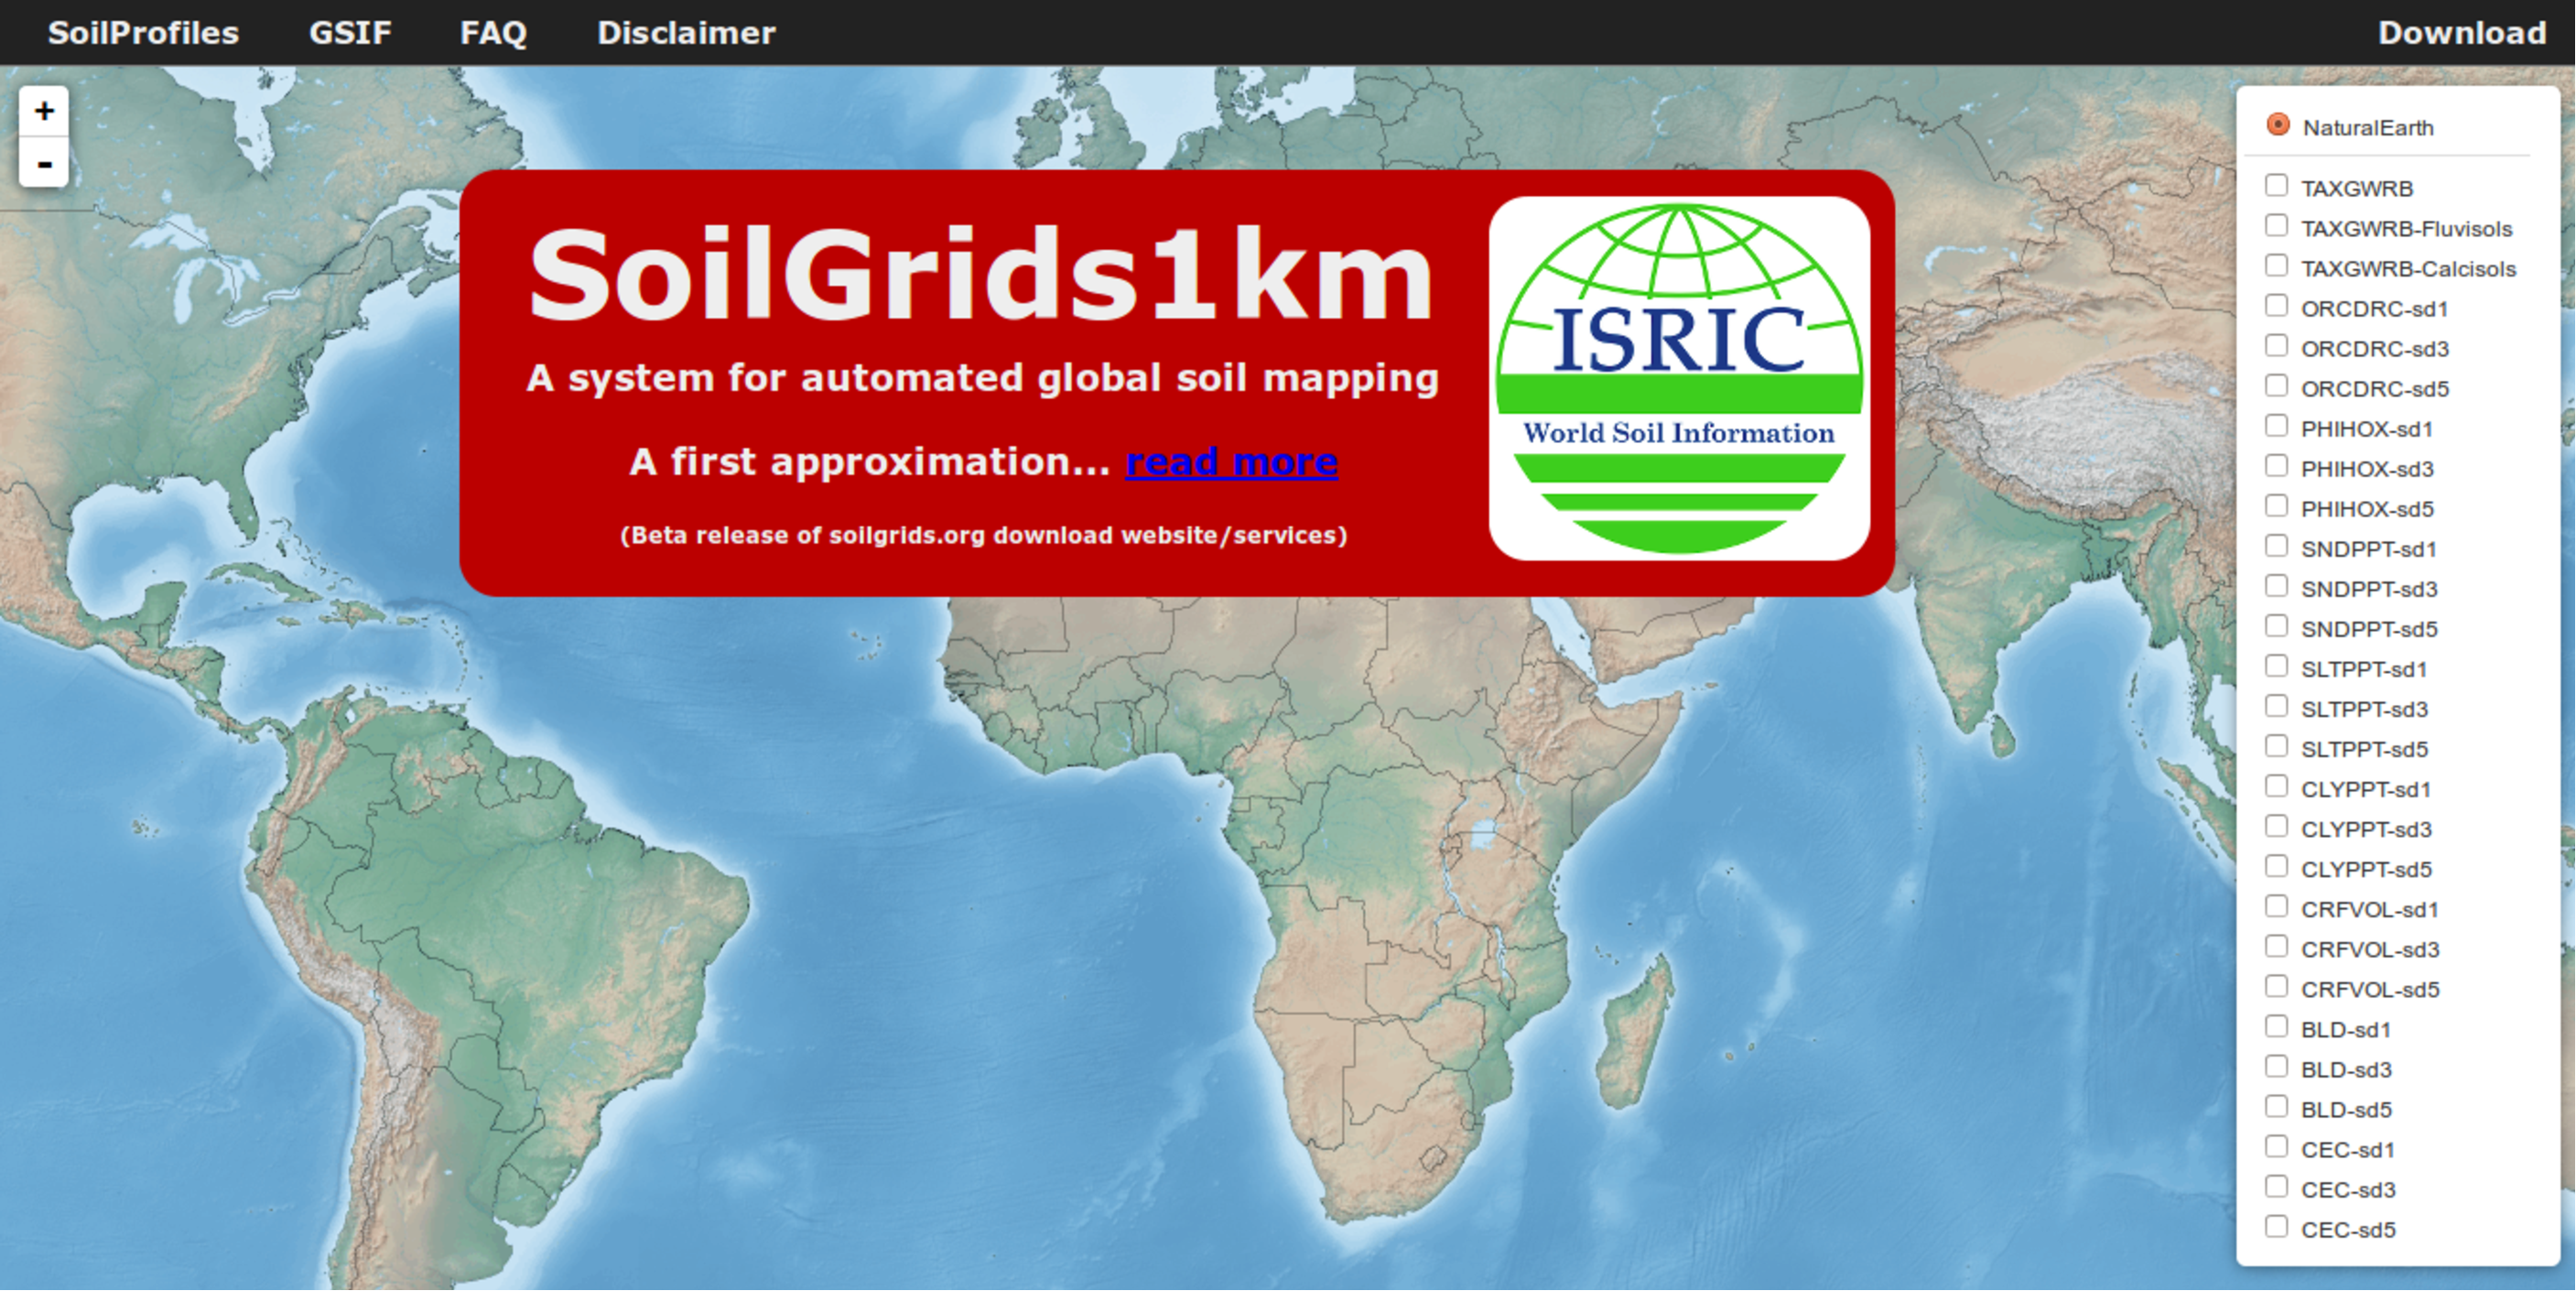
\includegraphics[width=\textwidth]{figuras/worldgrids}
 \caption{World Grids - mapas de solo para o mundo inteiro.}
 \label{fig:worldgrids}
\end{center}
\end{minipage}
\end{figure*}




Para gerar o mapa global da distribuição espacial das classes taxonômicas do WBR, os pesquisadores do ISRIC utilizaram os mapas de solos do Harmonized World Soil Database da FAO \citep{Fao2012} como covariáveis (variáveis explicativas). Tais mapas são constituídos por unidades de mapeamento que foram delineadas de maneira a definir regiões com características pedológicas e ambientais similares. É comum encontrar em cada unidade de mapeamento diversas classes taxonômicas de solo do WRB. Cada uma das classes taxonômicas possui uma estimativa do valor percentual de participação na composição da unidade de mapeamento. Em outras palavras, se uma unidade de mapeamento possui as classes taxonômicas Ferralsol e Lixisol com participação percentual de 70 e 30\%, então, se abrirmos 100 trincheiras, fizermos a descrição morfológica, coletarmos amostras e fizermos análises laboratoriais, 70 perfis serão classificados como Ferralsol, 30 perfis como Lixisol, e nenhum como, por exemplo, Planosol, ou Arenosol, ou Leptosol, e assim por diante.




Usando a nomenclatura estatística, o valor percentual de participação de uma classe taxonômica na composição da unidade de mapeamento constitui uma probabilidade (a probabilidade de ocorrência de uma determinada classe taxonômica). Esses valores podem ser usados para criar mapas da probabilidade de ocorrência de cada uma das classes taxonômicas em todo o mundo (veja mais em \url{worldgrids.org}). Por meio do uso de modelos de regressão logística (veja mais em \cite{tenCatenEtAl2011}), os pesquisadores do ISRIC foram capazes de relacionar dados de observações de campo (perfis de solo) com os mapas de probabilidade de ocorrência das classes taxonômicas do WRB, e predizer qual classe taxonômica do WRB é mais provável de ser encontrada em um determinado local.




Dois questionamentos podem ser elaborados quanto a produção de mapas de distribuição de classes taxonômicas de solo. O primeiro de cunho prático e o segundo teórico.




\begin{enumerate}
 \item Por que mapear classes taxonômicas? Qual é a finalidade prática dessa abordagem?
 \item Podemos mapear classes taxonômicas? Qual é a base conceitual que dá suporte à essa prática?
\end{enumerate}




De fato, ainda são poucas as experiências com o uso de mapas de classes taxonômicas do solo para fins de planejamento do uso do solo e das terras. Na grande maioria dos casos são utilizados mapas de solo com unidades de mapeamento delineadas em função de diversas características ambientais. Mas talvez existam exemplos de sucesso que desconhecemos porque não foram compartilhados. Assim, particularmente, acredito que a resposta ao primeiro questionamento só pode ser elaborada a partir do relato de experiências com tais mapas de solo. Em outras palavras, o método de raciocínio indutivo (veja mais na \href{http://pt.wikipedia.org/wiki/M\%C3\%A9todo\_indutivo}{Wikipédia}) parece ser o mais apropriado para elaborar uma resposta satisfatória. Já o segundo questionamento necessita de uma avaliação conceitual mais apurada. Talvez o método de raciocínio dedutivo (veja mais na \href{http://pt.wikipedia.org/wiki/M\%C3\%A9todo\_dedutivo}{Wikipédia}) seria o mais apropriado para tal situação. Na próxima seção forneço alguns elementos para auxiliar na discussão.




\section{Solo como Objeto, Imagem e Conceito}
\label{sec:conceito}




Segundo Igo Lepsch, o solo pode ser distinguido de três maneiras diferentes: como objeto, imagem e conceito (veja mais no \href{https://groups.google.com/forum/#!forum/soil-mapping}{Grupo de Discussão sobre Levantamentos Pedológicos Detalhados}). Tal distinção seria feita consciente ou inconscientemente. O solo como \textbf{objeto} seria uma realidade natural correspondente ao \textit{continuum} (por exemplo, o corpo de solo que um delineamento representa em um mapa pedológico detalhado). Já o solo como \textbf{imagem} seria a representação que fazemos do solo para nós mesmos depois de termos observado sua morfologia. Nesta representação somente as características mais marcantes são retidas, assim como em uma fotografia, onde podemos ver somente as feições externas de um corpo. Tal representação pode ser constituída, por exemplo, pela descrição que fazemos no caderno ou computador de campo, e pela foto do perfil de solo e da paisagem em que ocorre. Por fim, o solo como \textbf{conceito}, que não teria existência real por consistir de um indivíduo teórico ou táxon (classe taxonômica) de uma classificação que mais se aproxima de nossa imagem do solo. Em outras palavras, um \textit{Latossolo Vermelho Distrófico} - um subgrupo do Sistema Brasileiro de Classificação de Solos - por exemplo, não constitui um objeto na natureza, mas sim um conceito que usamos para representar nossa percepção sobre uma determinada realidade (um perfil de solo que descrevemos em uma determinada paisagem).




Vou tentar deixar as coisas mais claras e usar um exemplo dado por Igo Lepch. Quando estamos no campo realizando um levantamento de solos, observamos a superfície e o perfil do solo na parede de uma trincheira. Estaria aí nosso solo como \textbf{objeto}. Em seguida, capturamos algumas imagens com nossa câmera, descrevemos a sua aparência (cor, número e sequência de horizontes, textura e transição entre os horizontes, profundidade, etc) e registramos suas coordenadas geográficas. Estaria aí nosso como \textbf(imagem). De posse da imagem que temos do solo e dos dados analíticos de laboratório, agora no conforto de nosso escritório, identificamos esse solo como sendo um \textit{Latossolo Vermelho Distrófico}. Estaria aí nosso solo como \textbf{conceito}.




Se adotarmos a perspectiva de que um levantamento de solos deve resultar em um mapa que representa objetos reais, então uma mapa de classes taxonômicas de solo segundo um determinado sistema de classificação não possui fundamentação conceitual. Os objetos reais são definidos aqui como os corpos de solo, enquanto as classes taxonômicas têm apenas existência conceitual, isto é, são abstrações da mente humana.




\section{É Possível Mapear \textit{Abstrações}?}
\label{sec:abstraction}




Podemos mapear classes taxonômicas? Qual é a base conceitual que dá suporte à essa prática? O raciocínio dedutivo apresentado acima nos leva a responder negativamente à este questionamento, afirmando que não existe base conceitual que dê suporte ao mapeamento de classes taxonômicas. Em suma, seria impossível mapear \textit{abstrações}. Mas faltam-me exemplos práticos de aplicação de mapas de classes taxonômicas e o relato de outros profissionais para que possa acoplar dedução e indução para chegar a uma resposta que me seja satisfatória. É por esse motivo que lanço os dois questionamentos feitos no início deste artigo ao profissionais que atuam no mapeamento de solos, e acrescento:




\begin{itemize}
 \item É possível mapear abstrações?
\end{itemize}




Àqueles que sentirem-se desafiados, peço que enviem sua opinião para o endereço de e-mail \email{pedometria.news@gmail.com} até o final do mês de abril para que sejam publicadas na próxima edição de \textit{Pedometria}.




\begin{footnotesize}
\begin{thebibliography}{99}




\bibitem[IUSS WORKING GROUP WRB(2007) IUSS WORKING GROUP WRB]{fao2007}
IUSS WORKING GROUP WRB (2007)
\newblock {\em World reference base for soil resources 2006 - A framework for international classification, correlation and communication, first update 2007}.
\newblock Rome: FAO, 116p.




\bibitem[FAO/IIASA/ISRIC/ISS-CAS/JRC(2012) FAO/IIASA/ISRIC/ISS-CAS/JRC]{Fao2012}
FAO/IIASA/ISRIC/ISS-CAS/JRC (2012)
\newblock {\em Harmonized World Soil Database}.
\newblock Roma: FAO / Luxemburgo: IIASA, 42p.




\bibitem[Rossiter(2000) Rossiter]{Rossiter2000}
Rossiter, D.G. (2000)
\newblock {\em Methodology for soil resource inventories}.
\newblock Enschede: Faculty of Geo-Information Science and Earth Observation - University of Twente, 132p.




\bibitem[ten Caten et~al.(2011) ten Caten, Dalmolin, Pedron, Mendonça-Santos]{tenCatenEtAl2011}
ten Caten, A., Dalmolin, R.S.D., Pedron, F.A., Mendonça-Santos, M.L. (2011)
\newblock Multiple Logistic Regressions: controlling factors in applications to soil class prediction.
\newblock {\em Revista Brasileira de Ciência do Solo} 35: 53-62.




\end{thebibliography}
\end{footnotesize}




\address{Alessandro Samuel-Rosa\\
\footnotesize
UFRRJ e ISRIC-World Soil Information\\
\url{www.soil-scientist.net}\\
\email{alessandro-rosa@wur.com}}




%%% Local Variables:
%%% mode: latex
%%% TeX-master: 3rd-edition.tex
%%% End:
